\documentclass[a4paper, 10pt]{article}

\usepackage[english]{babel}
\usepackage[T1]{fontenc}
\usepackage[utf8]{inputenc}
\usepackage{textcomp}
\setlength{\marginparwidth}{2cm}

\usepackage{comment}
\usepackage{todonotes}

\usepackage{amsmath}
\usepackage{amssymb}
\usepackage{latexsym}
\usepackage{bm}

\usepackage{enumitem}
\usepackage{array}
\setlength\extrarowheight{5pt}

\usepackage{xcolor}
\usepackage{graphicx}
\graphicspath{ {./img/} }

\newcommand\scalemath[2]{\scalebox{#1}{\mbox{\ensuremath{\displaystyle #2}}}}

\usepackage{hyperref}
\usepackage{listings}
\usepackage{color}
\definecolor{dkgreen}{rgb}{0,0.6,0}
\definecolor{gray}{rgb}{0.5,0.5,0.5}
\definecolor{mauve}{rgb}{0.58,0,0.82}
\lstset{frame=tb,
    language=Python,
    aboveskip=3mm,
    belowskip=3mm,
    showstringspaces=false,
    columns=flexible,
    basicstyle={\small\ttfamily},
    numbers=none,
    numberstyle=\tiny\color{gray},
    keywordstyle=\color{blue},
    commentstyle=\color{dkgreen},
    stringstyle=\color{mauve},
    breaklines=true,
    breakatwhitespace=true,
    tabsize=3
}

\title{Homework Assignment N°2}
\author{AML3\\Thibault Douzon\\Georgios Lioutas}
\date{December 15th, 2018}

\begin{document}
\maketitle

\pagebreak

\tableofcontents

\pagebreak
\section{Exercise 1}
\subsection{Part a}
From the topology of the graph, we deduce that:
$$
P(S) = \sum_c P(D\vert C=c) \sum_d P(I\vert D=d) \sum_i P(S\vert I=i) \sum_g P(G=g\vert D=d, I=i)
$$
Because $P(G\vert D=d, I=i)$ is a probabitlity distribution, $\sum_g P(G\vert D=d, I=i) = 1$.
Our final formula is the following:
$$
P(S) = \sum_c P(D\vert C=c) \sum_d P(I\vert D=d) \sum_i P(S\vert I=i)
$$
$$
P(S) = \left[s_0, s_1\right] = \left[0.516, 0.484\right]
$$
\subsection{Part b}
From the graph we know that
$$
P(G, I=i_0) = \sum_c P(D\vert C=c) \sum_d P(I\vert D=d) P(G\vert D=d, I=i0) \sum_s P(S\vert I=i_0) 
$$
Once again, $P(S\vert I=i_0)$ is a probability distribution, then
$$
P(G, I=i_0) = \sum_c P(D\vert C=c) \sum_d P(I\vert D=d) P(G\vert D=d, I=i0)
$$
$$
P(G, I=i_0) = \left[p(g_0\vert i_0), p(g_1\vert i_0), p(g_2\vert i_0)\right] = \left[0.1384, 0.2272, 0.2024\right]
$$
Because it is not a probability distribution, its sum is not 1. From Bayes rule we know that by dividing by 
$P(I=i_0)$ we would obtain $P(G\vert I=i_0)$ which is a distribution.
$$
P(G\vert I=i_0) = \frac{P(G,I=i_0)}{P(I=i_0)} = \frac{P(G,I=i_0)}{\sum_g P(G,I=i_0)} = \frac{P(G,I=i_0)}{0.568}
$$
$$
P(G\vert I=i_0) =\left[0.244, 0.4, 0.356\right]
$$
Which adds up to 1 accordingly.
\subsection{Part c}
Same process as before:
$$
P(S, G=g_0) = \sum_c P(D\vert C=c) \sum_d P(I\vert D=d) \sum_i P(G=g_0\vert D=d, I=i) P(S\vert I=i)
$$
$$
P(S, G=g_0) = \left[p(s_0\vert g_0), p(s_1\vert g_0)\right] = \left[0.245, 0.148\right]
$$
Because it is not a probability distribution, its sum is not 1. From Bayes rule we know that by dividing by 
$P(G=g_0)$ we would obtain $P(S\vert G=g_0)$ which is a distribution.
$$
P(S\vert G=g_0) = \frac{P(S,G=g_0)}{P(G=g_0)} = \frac{P(S,G=g_0)}{\sum_s P(S,G=g_0)} = \frac{P(S,G=g_0)}{0.393}
$$
$$
P(S\vert G=g_0) =\left[0.624,0.376\right]
$$
Which adds up to 1 accordingly.
\section{Exercise 2}
In this exercise, the graph represents a Markov network. The function $\Phi$ is given by the 
different tables of values.
$$
\Phi(C,D,I,G,S) = \Phi(C) \times \Phi(C,D) \times \Phi(D,I) \times \Phi(D,I,G) \times \Phi(I,S)
$$
To get a specific value of $\Phi$ for a given parameter, we need to marginalize over all other
possible parameters.
\\
To compute probabilities we must then normalize $\Phi$ by the constant $Z$ such as:
$$
Z = \sum_X \Phi(X)
$$
where $X$ takes all possible joint probabilities.
$$
Z = \sum_c \sum_d \sum_i \sum_g \sum_s \phi(C=c, D=d, I=i, G=g, S=s) = 69200
$$
\subsection{Part a}
We first compute $\Phi(S)$:
$$
\Phi(S) = \left[\Phi(s_0), \Phi(s_1)\right] = \sum_c \sum_d \sum_i \sum_g \phi(C=c, D=d, I=i, G=g, S)
$$
$$
\Phi(S) = \left[25840, 43360\right]
$$
Now we can compute the probability $P(S)$:
$$
P(S) = \Phi(S)/Z = \left[0.373, 0.627\right]
$$
\subsection{Part b}
We now want to compute $\Phi(G, I=i_0)$. With the same formula as before:
$$
\Phi(G, I=i_o) = \sum_c \sum_d \sum_s \Phi(C=c, D=d, I=i_o, G, S=s) = \left[13680, 19680, 15840\right]
$$
The corresponding probability $P(G, I=i_0)$:
$$
P(G, I=i_o) = \frac{1}{Z} \sum_c \sum_d \sum_s \Phi(C=c, D=d, I=i_o, G, S=s) = \left[0.198, 0.284, 0.229\right]
$$
And now using Baye's rule we can finally obtain the probability distribution $P(G\vert I=i_0)$:
$$
P(G\vert I=i_0) = \frac{P(G, I=i_0)}{P(I=i_0)} = \frac{P(G, I=i_0)}{\sum_g P(G, I=i_0)}
$$
$$
P(G\vert I=i_0) = \left[0.278, 0.4, 0.322\right] 
$$
\subsection{Part c}
We now want to compute $\Phi(S, G=g_0)$. With the same formula as before:
$$
\Phi(S, G=g_o) = \sum_c \sum_d \sum_i \Phi(C=c, D=d, I=i, G=g_0, S) = \left[12640, 13420\right]
$$
The corresponding probability $P(S, G=g_0)$:
$$
P(S, G=g_o) = \frac{1}{Z} \sum_c \sum_d \sum_i \Phi(C=c, D=d, I=i, G=g_0, S) = \left[0.183, 0.194\right]
$$
And now using Baye's rule we can finally obtain the probability distribution $P(S\vert G=g_0)$:
$$
P(S\vert G=g_0) = \frac{P(S, G=g_0)}{P(G=g_0)} = \frac{P(S, G=g_0)}{\sum_s P(S, G=g_0)}
$$
$$
P(S\vert G=g_0) = \left[0.485, 0.515\right] 
$$

\section{Exercise: Message Passing}
\subsection{Part a}
To use sum-product algorithm, our graph needs to be a tree. Thus it is impossible to keep
both $\Phi(D,I)$ and $\Phi(D,I,G)$. We need to combine them together into one single factor node.
\\
Our factor graph is the following:
\begin{center}
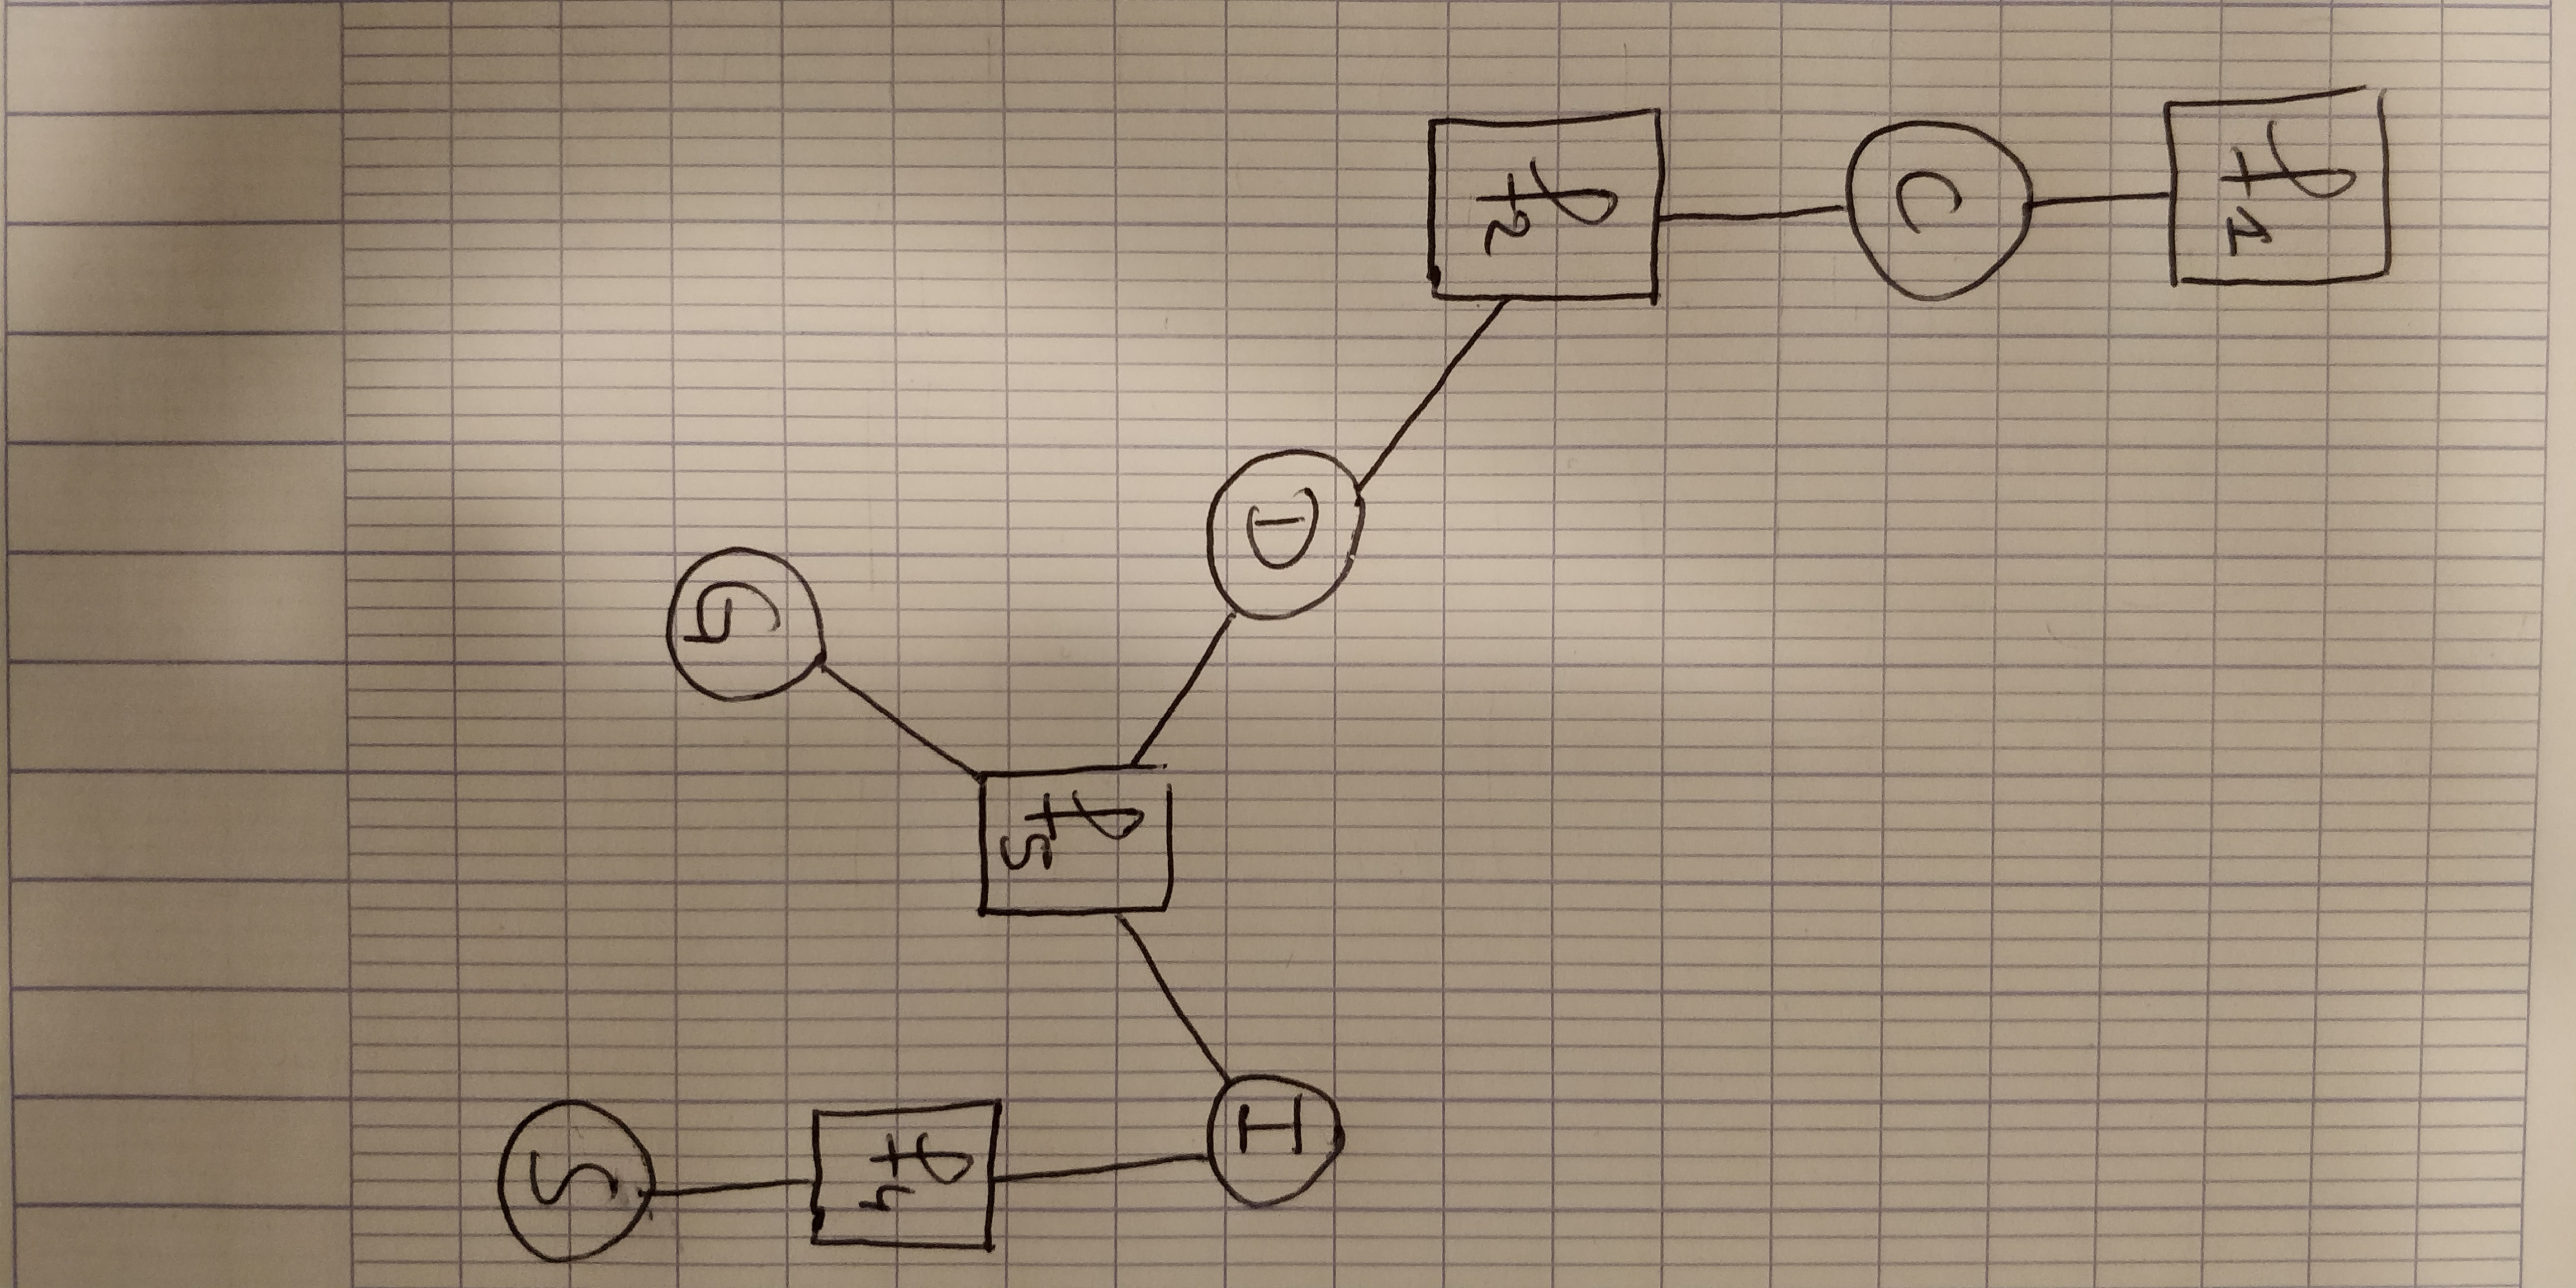
\includegraphics[angle=90,scale=0.06]{graph1}
\end{center}
The factor $f_5$ is the combination of $\Phi(D,I)$ and $\Phi(D,I,G)$. 
\\
It is computed as follows: for every set of value for the variables, multiply together $\Phi(D,I)$ and $\Phi(D,I,G)$.
We finally obtain the result table:
\begin{center}
\begin{tabular}{ |c|c|c|c| }
    \hline
    $f_5$ & $g_0$ & $g_1$ & $g_2$ \\
    \hline
    $d_0,i_0$ & 2 & 8 & 10\\
    \hline
    $d_0,i_1$ & 8 & 8 & 4\\
    \hline
    $d_1,i_0$ & 18 & 24 & 18\\
    \hline
    $d_1,i_1$ & 14 & 4 & 2\\
    \hline
\end{tabular}
\end{center}
\subsection{Part b}
We now want to compute the probability $P(S)$ using message passing.
Node S is now the root of the tree and we start apply message passing from the leaves.
\begin{enumerate}
    \item $\mu_{f_1\rightarrow C} = \Phi(C) = \left[3, 7\right]$
    \item $\mu_{C\rightarrow f_2} = \Phi(C) = \left[3, 7\right]$
    \item $\mu_{f_2\rightarrow D} = \Phi(C,D) = \left[3\times 2+ 7\times 3, 3\times 8 + 7 \times 7\right] = \left[27, 73\right]$
    \item $\mu_{D\rightarrow f_5} = \left[27, 73\right]$
    \item $\mu_{G\rightarrow f_5} = \left[1, 1\right]$
    \item $\mu_{f_5\rightarrow I} = \sum_d \sum_g  {\mu_{D\rightarrow f_5}}_d \times {\mu_{G\rightarrow f_5}}_g \times f_5(d,g) = \left[4920, 2000\right]$
    \item $\mu_{I\rightarrow f4} = \left[4920, 2000\right]$
    \item $\mu_{f4\rightarrow S} = \Phi(S) = \left[2\times4920+8\times2000, 8\times4920+2\times2000\right] = \left[25840, 43360\right]$
\end{enumerate}
We can now normalize our last result to obtain a probability distribtution:
$$
P(S) = \left[0.373, 0.627\right]
$$
Which is the same result as in Exercise 2.
\subsection{Part c}
We now want to compute $P(G\vert I=i_0)$ also using message passing.
Because we observe that $I=i_0$, we need to add a factor node to the graph signifying
that the variable $I$ is constrained to the value $i_0$. 
\\
We do so by adding a factor node $f_6$ only linked to $I$ with the follow table of values:
\begin{center}
\begin{tabular}{ |c|c|c| }
    \hline
    $f_6$ & $i_0$ & $i_1$ \\
    \hline
          & 1 & 0 \\
    \hline
\end{tabular}
\end{center}
It expresses the fact $i_0$ prevails over $i_1$.
\\
Our factor graph is now the following:
\begin{center}
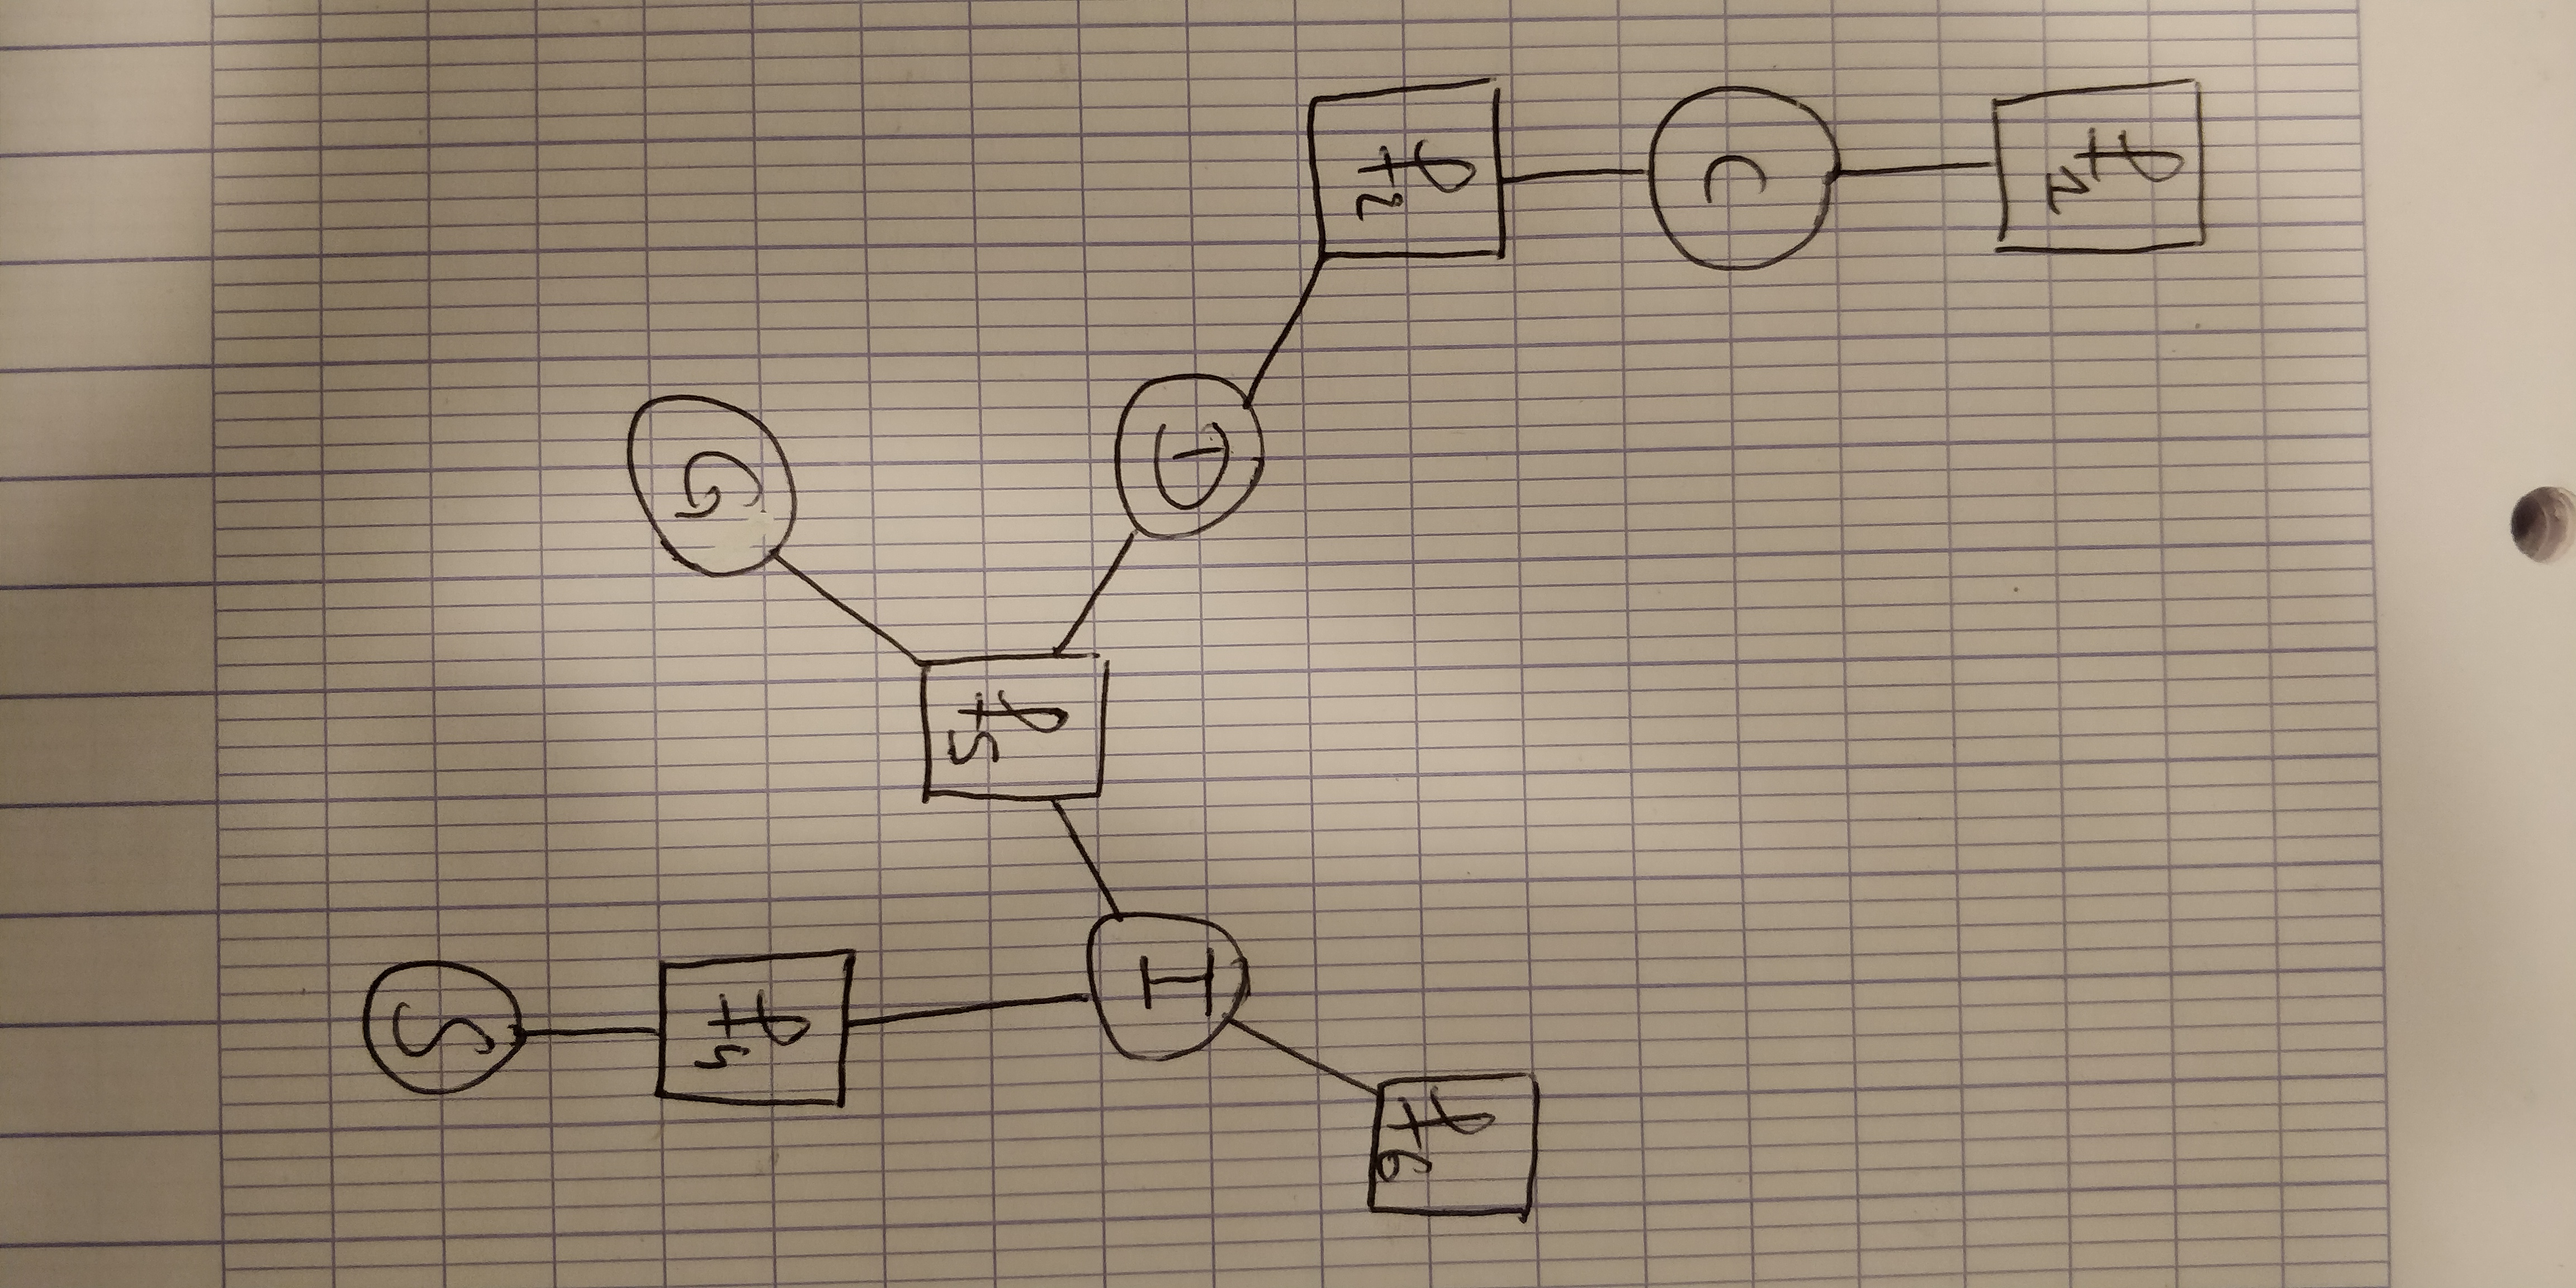
\includegraphics[angle=90, scale=0.06]{graph2}
\end{center}
To apply the message passing, $G$ is now the root of the tree. The messages starting at $f_1$
will be the same as in the last question until ther get to $f_5$.
\begin{enumerate}
    \item $\mu_{f_1\rightarrow C} = \Phi(C) = \left[3, 7\right]$
    \item $\mu_{C\rightarrow f_2} = \Phi(C) = \left[3, 7\right]$
    \item $\mu_{f_2\rightarrow D} = \Phi(C,D) = \left[3\times 2+ 7\times 3, 3\times 8 + 7 \times 7\right] = \left[27, 73\right]$
    \item $\mu_{D\rightarrow f_5} = \left[27, 73\right]$
    \item $\mu_{S\rightarrow f_4} = \left[1, 1\right]$
    \item $\mu_{f_4\rightarrow I} = \left[1\times2+1\times8, 1\times8 + 1\times 2\right] = \left[10, 10\right]$
    \item $\mu_{f_6\rightarrow I} = \left[1, 0\right]$
    \item $\mu_{I\rightarrow f_5} = \left[1\times10, 0\times10\right] = \left[10, 0\right]$
    \item $\mu_{f_5\rightarrow G} = \sum_d \sum_i  {\mu_{D\rightarrow f_5}}_d \times {\mu_{I\rightarrow f_5}}_g \times f_5(d,i) = \left[13680, 19680, 15840\right]$
\end{enumerate}
To obtain a probability distribution, we just have to normalize:
$$
P(G\vert I=i_0) = \left[0.278, 0.4, 0.322\right]
$$
Which is again the same as in the previous exercise.
\end{document}
